\chapter{Fundamentação Teórica}
\label{ch:fundamentacao}
\par Neste capítulo ser\~ao fundamentados os conhecimentos b\'asicos para o entendimento do trabalho.

\section{Recursos assistivos}

\par No Brasil, pessoas que possuem algum tipo de deficiência tem o direito de receber tratamento especial em diferentes meios e serviços \cite{ANDRIOLI2017}, para que a dignidade e necessidades básicas do individuo sejam garantidas \cite{DeOliveira2011}. Uma das formas de garantir este direito a pessoas com deficiência é através da aplicação de Tecnologias Assistivas.

\par Tecnologia assistiva é o termo que identifica todo o arsenal de recursos e serviços assistivos \cite{Bersch2017}, sendo, os recursos assistivos tudo aquilo que é produzido para aumentar, manter ou melhorar as capacidades de pessoas com deficiência \cite{tonollijoseberschrita2017} e os serviços representam tudo o que ajuda na aplicação e utilização de recursos assistivos \cite{tonollijoseberschrita2017}.

\par De acordo com \citeonline{tonollijoseberschrita2017} existem diferentes tipos de TAs, sendo algumas delas: recursos de acessibilidade ao computador, auxílios para surdos ou com déficit auditivo e auxílios para a vida diária.

\par Todos esses recursos podem ser construídos através da aplicação de diferentes técnicas e métodos. Por exemplo, para o caso de uma pessoa que possua deficiência auditiva e necessita de um atendimento especial para seu processo de aprendizagem, é possível criar recursos assistivos que facilitem o aprendizado e comunicação através de pranchas de comunicação \cite{Bersch2017}. Também pode ser aplicado, formas de comunicação através da Língua Brasileira de Sinais (Libras), uma língua manuo-motora de recepção visual, ou seja, através de sinais e gestos criam-se representações de letras e palavras (Figura \ref{figure:sinslibras}), sendo a mais usada pelos surdos no Brasil \cite{paulovazdecarvalho2019} e é reconhecida oficialmente nos meios legais segundo a Lei n° 10.436, de 25 de Abril de 2002. Além disso, seu uso em RAs pode ser feito para acessibilidade, uma vez que, boa parte dos surdos não são alfabetizados na Língua Portuguesa, somente em Libras \cite{tve2016}.

\image{0.50}{bom-dia-boa-tarde-noite-saudacoes-em-libras-surdos.jpg}{Exemplos de sinais de Libras}{figure:sinslibras}{\citeonline{markewiczpaulamaria2017}}

\par Os exemplos de RAs listados acima podem ser recursos desenvolvidos para \textit{tablets}, celulares e aplicações \textit{web} e não somente, em certos casos, simples representações em papel, ou mesmo em um brinquedo \cite{Bersch2017}, podem ser considerados RAs.

\section{Regressão linear}

\par Análise de regressão é uma técnica preditiva \cite{introDataMining2009} que tem com objetivo modelar a relação funcional entre uma variável dependente e uma ou mais variáveis independentes \cite{Peternelli2003}. Assim, verifica-se a variação de uma variável, decorrente a variação de outra variável \cite{Peternelli2003, mannprems2006}.

\par Essa relação funcional pode ser apresentada de diversas formas: linear, quadrática, cúbica, dentre outras \cite{Peternelli2003}. A representação de cada um desses comportamentos é feita através de modelos matemáticos \cite{mannprems2006}.

\par A regressão linear, por exemplo, é a representação de uma relação funcional linear entre duas variáveis, sendo essas, a variável dependente, que representa a variável que está sendo explicada e as variáveis independentes que explicam a variável independente \cite{mannprems2006}. 

\par Uma das formas de representação deste modelo é apresentado na Equação \ref{form:linearregression}. 
\begin{equation}
    \widehat{y} = a + bx
\label{form:linearregression}
\end{equation}

\par Onde, $ \widehat{y} $ é a variável dependente, que está sendo explicada, \textit{x} a variável independente, \textit{a} é o termo constante e \textit{b} é a inclinação. Sendo que, \textit{x} e \textit{y} representam os coeficientes de regressão, que são modificados para que a relação funcional entre as variáveis sejam explicadas \cite{introDataMining2009}.

\par No momento em que as coeficientes de regressão são ajustados e fazem a representação do comportamento entre duas ou mais variáveis, como citado acima, passa a ser possível a sua aplicação para a predição de novos valores \cite{introDataMining2009}, esses que ao serem preditos terão o mesmo padrão de comportamento do conjunto de dados aplicado para a criação dos coeficientes.

\section{Inteligência artificial}

\par Sistemas inteligentes de forma geral são aqueles que apresentam a capacidade de planejar e resolver problemas através de dedução e indução utilizando conhecimentos de situações anteriores \cite{VonZuben2013}, e a inteligência artificial, é um campo da ciência e engenharia de computação \cite{VonZuben2013} que possibilitam a sistemas computacionais, perceber, raciocinar e agir \cite{Winston1992}.

\par As técnicas computacionais mais utilizadas para o desenvolvimento e aplicação de inteligência artificial, são aquelas relacionadas ao aprendizado de máquina. Esta que é uma área que tem como objetivo principal, desenvolver técnicas que permitam aos sistemas adquirir conhecimento de forma automática e com estes conhecimentos tomar decisões \cite{Augusto2007}.

\par Para a realização do aprendizado de máquina, existem diversas técnicas, que vão de simples regressões estatísticas, até modelos complexos, como às redes neurais artificiais \cite{andrewngcourse}.

\section{Redes neurais artificiais}

\par Redes neurais artificiais são sistemas computacionais que busca modelar o sistema cerebral natural humano, estas que são uma das formas de soluções de problemas apresentados dentro do âmbito de inteligência computacional \cite{Cintra2019}.

%% Não creio que isto esteja escrito da melhor forma, mas está melhor que o texto inicial (01/02/2019)
% Escrever mais!! Fale sobre machine learning aqui tbm -> As referências do Deep Learning with R são boas ! (13/03/2019)
\par Por buscar modelar o cérebro humano, as RNAs utilizam como unidade básica de processamento, os neurônios artificiais \cite{Haykin2001}, da mesma forma que o cérebro utiliza os neurônios biológicos. % Preciso criar um complemento para ir para o próximo capítulo ? (01/02/2019)

\subsection{Neurônio biológico}

\par Todo o processamento de informações no cérebro humano, é feito através de elementos biológicos de processamento, que operam em paralelo para a produção de ações apropriadas para cada estímulo recebido pelo corpo. A célula base do sistema nervoso cerebral é o neurônio (Figura \ref{figure:bioneuron}), e sua principal função é conduzir impulsos (Representando os estímulos) levando em consideração as condições do corpo e assim produzindo ações. Os neurônios também são os responsáveis pelos atos do pensamento e armazenamento de informações \cite{livroNunes2016}.

\par Os neurônios podem ser divididos em três partes elementares, os dendritos, que captam de forma continua os impulsos vindos de outros neurônios, o corpo celular, que processa todas as informações captadas e os axônios que enviam as informações processadas no corpo celular para outros neurônios.

\image{1.4}{neuronio-biologico.png}{Ilustração do neurônio biológico}{figure:bioneuron}{\citeonline{Remes2016}}

\par Estima-se que a rede neural cerebral, possui cerca de 100 bilhões de neurônios, cada um desses mantendo conexão com uma média de 6.000 outros neurônios, gerando cerca de 600 trilhões de conexões \cite{shepherdgordonm1990}. A região de conexão entre os neurônios são chamadas de sinapses, que exercem ponderações entre as conexões entre os neurônios, fazendo assim com que haja regiões do cérebro especializadas em diferentes tarefas.

\par A representação inicial deste conjunto de neurônios em sistemas de computação foi implementada através de circuitos eletrônicos, apresentado por \citeonline{McCullochS1943}, estes que foram utilizados como base para a criação dos modelos de neurônios artificiais apresentados por \citeonline{Hodgkin1952}.

\subsection{Neurônio artificial}

\par Como citado anteriormente, os neurônios artificiais, são modelos computacionais para a representação do neurônio biológico nas RNAs, e da mesma forma que em um neurônio biológico, a representação deste é feita com três elementos básicos \cite{Haykin2001}:  

\begin{itemize}
	\item Conjunto de sinapses, cada uma caracterizada por um peso, este que indica a relevância de cada valor de entrada;
	\item Somador, ou combinador linear, que faz a ponderação dos valores de entrada com as respectivas sinapses do neurônio;
	\item Função de ativação utilizada para restringir os valores de saída do neurônio.
\end{itemize}

\par Ainda de acordo com \citeonline{Haykin2001}, a estes modelos neuronais pode-se aplicar um \textit{bias}, este que será o responsável pelo aumento ou diminuição dos valores de entrada da função de ativação. Em termos matemáticos, pode-se descrever um neurônio k (Figura \ref{fig:modelo_neuronio}) com as seguintes equações \cite{Haykin2001}:

\begin{equation}
	u_{k} = \sum_{j=1}^{n} w_{kj} x_{j}
\end{equation}
e
\begin{equation}
	y_{k} = f(u_{k} + b_{k})	
\end{equation}
onde $ x_{1}, x_{2}, ..., x_{n} $ são os sinais de entrada; $ w_{k1}, w_{k2}, ..., w_{kn} $ são os pesos sinápticos do neurônio k; $ u_{k} $ é a saída do combinador linear; $ b_{k} $ é o \textit{bias}; $ f(u_{k} + b_{k}) $ a função de ativação; e $ y_{k} $ representa a saída do neurônio.

\begin{figure}[H]
    \centering
    \caption{Neurônio Artificial}
    \begin{tikzpicture}[
init/.style={
  draw,
  circle,
  inner sep=2pt,
  font=\Huge,
  join = by -latex
},
init2/.style={
  draw,
  circle,
  inner sep=2pt
},
neuron missing/.style={
    draw=none, 
    scale=4,
    text height=0.333cm,
    execute at begin node=\color{black}$\vdots$
  },
squa/.style={
  draw,
  inner sep=2pt,
  font=\Large,
  join = by -latex
},
squa2/.style={
  draw,
  inner sep=2pt,
  font=\Large
},
start chain=2,node distance=13mm
]
\node[on chain=2] 
  (x2) {$x_2$};
%\node[below of=x2] (dots) {$\vdots$} -- (dots) node[right of=dots] (ldots) {$\vdots$};
%\node[below of=2] (dots) {$\vdots$} -- (dots) node[left of=dots] (ldots) {$\vdots$};
\node[on chain=2,init2,join=by o-latex] 
  {$w_{k2}$};
\node[on chain=2,init] (sigma)
  {$\displaystyle\Sigma$};
\node[on chain=2,squa2,label=above:{\parbox{2cm}{\centering Função de \\ ativação}}](te) {$f$};
\node[on chain=2,label=above:Saída] (sa)
  {$y_k$};
\begin{scope}[start chain=1]
\node[on chain=1] at (0,1.5cm) 
  (x1) {$x_1$};
\node[on chain=1,init2,join=by o-latex] 
  (w1) {$w_{k1}$};
\end{scope}
\begin{scope}[start chain=3]
\node[on chain=3] at (0,-1.5cm) 
  (x3) {$x_n$};
\node[on chain=3, init2,label=below:{\parbox{2cm}{\centering Pesos \\ sinápticos}},join=by o-latex] 
  (w3) {$w_{kn}$};
\end{scope}
\node[label=above:\parbox{2cm}{\centering Bias \\ $b$}] at (sigma|-w1) (b) {};

\draw[-latex] (w1) -- (sigma);
\draw[-latex] (w3) -- (sigma);
\draw[o-latex] (b) -- (sigma);
\draw[-latex] (sigma) -- (te) node[midway,sloped, above]{$v_k$};
\draw[-latex] (te) -- (sa) node[midway,sloped, above]{};
\draw[decorate,decoration={brace,mirror}] (x1.north west) -- node[left=10pt] {Entradas} (x3.south west);
\end{tikzpicture}
    \fonte{Adaptado de \citeonline{Haykin2001}}
    \label{fig:modelo_neuronio}
\end{figure}

\par A partir da Figura \ref{fig:modelo_neuronio} é possível realizar uma comparação entre cada um dos elementos do neurônio artificial e biológico. Os sinais de entrada, advindos do meio externo, normalmente uma aplicação, são análogos aos impulsos elétricos captados pelos dendritos no neurônio biológico.  Os pesos sinápticos representam a importância do sinal recebido para o neurônio, o que representa as ponderações exercidas pelas junções sinápticas do modelo biológico, ou seja, a força do caminho entre as sinapses, citados anteriormente. O campo de somatório junto a função de ativação, representam o corpo celular do neurônio biológico, é nesta parte que os resultados criados pelo neurônio são calculados \cite{livroNunes2016} 

\subsection{Arquiteturas de rede} 

\par Para \citeonline{livroNunes2016} uma RNA pode ser constituída de até três partes diferentes, estas denominadas de camadas, as quais são nomeadas a seguir:

\begin{itemize}
    \item Camada de entrada: É a camada responsável pelo recebimento de dados;
    \item Camadas escondidas, intermediárias ou ocultas: São camadas compostas de neurônios responsáveis pela extração de características associadas ao processo ou sistema;
    \item Camadas de saída: Também constituída de neurônios, esta camada é responsável pela produção e apresentação dos resultados finais da rede.
\end{itemize}

\par Das camadas descritas acima, devem estar presentes em uma RNA no mínimo a camada de entrada e a camada de saída \cite{Cintra2019}.

\par Diferentes formas de organização de cada uma destas camadas, especialmente relacionadas a forma de relação entre os neurônios, definem as arquiteturas de RNA \cite{livroNunes2016}. \citeonline{Haykin2001} define a existência de duas classes de arquiteturas fundamentais, sendo elas: Redes de alimentação direta, com uma ou várias camadas e Redes recorrentes.

\par As redes de alimentação direta, são denominadas desta forma por conta de seu fluxo percorrer uma única direção \cite{Cintra2019}, iniciando o fluxo na camada de entrada seguindo pelas diferentes camadas até o neurônio de saída. Este tipo de rede pode possuir uma ou várias camadas ocultas.

\par Para as redes de alimentação direta com uma única camada, tem-se como tipo comum a \textit{Perceptron} (Figura \ref{figure:camadaunida}). Em sua estrutura são apresentadas duas camadas, entrada e saída, porém são nomeadas de camada única já que existem operações matemáticas ocorrendo apenas na camada de saída \cite{livroNunes2016}.

\begin{figure}[H]
    \centering
    \def\layersep{2.5cm}
    \caption{Rede de alimentação direta de camada única}
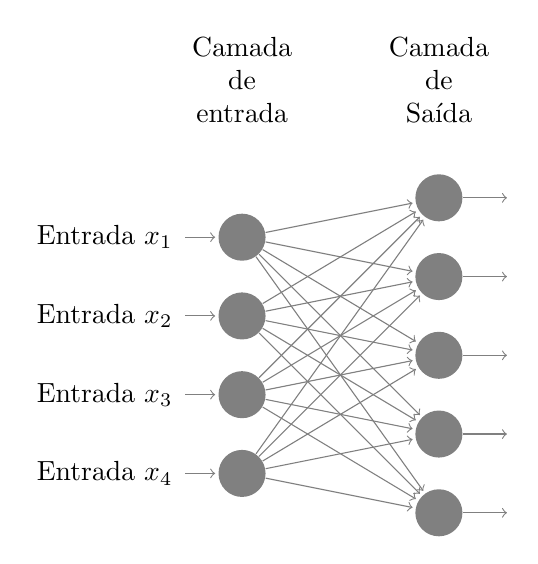
\begin{tikzpicture}[shorten >=1pt,->,draw=black!50, node distance=\layersep]
    \tikzstyle{every pin edge}=[<-,shorten <=1pt]
    \tikzstyle{neuron}=[circle,fill=black!25,minimum size=17pt,inner sep=0pt]
    \tikzstyle{input neuron}=[neuron, fill=black!50];
    \tikzstyle{output neuron}=[neuron, fill=black!50];
    \tikzstyle{hidden neuron}=[neuron, fill=black!50];
    \tikzstyle{annot} = [text width=4em, text centered]
    \tikzset{normal arrow/.style={draw,-triangle 45,very thick}}

    % Draw the input layer nodes
    \foreach \name / \y in {1,...,4}
    % This is the same as writing \foreach \name / \y in {1/1,2/2,3/3,4/4}
        \node[input neuron, pin=left:Entrada $x$$_\y$] (I-\name) at (0,-\y) {};

    % Draw the hidden layer nodes
    \foreach \name / \y in {1,...,5}
        \path[yshift=0.5cm]
            node[hidden neuron] (H-\name) at (\layersep,-\y cm) {};

    % Draw the output layer node
    %\node[output neuron,pin={[pin edge={->}]right:Saída}, right of=H-3] (O) {};

    % Connect every node in the input layer with every node in the
    % hidden layer.
    \foreach \source in {1,...,4}
        \foreach \dest in {1,...,5}
            \path (I-\source) edge (H-\dest);
            

    % Connect every node in the hidden layer with the output layer
    \foreach \source in {1,...,5}
        \draw[->] (H-\source) -- +(0.9,0);
        %\path (H-\source)  -- ();
        %\draw [->] (0,0) -- (30:20pt); 

    % Annotate the layers
    \node[annot,above of=H-1, node distance=1.5cm] (hl) {Camada de \\ Saída};
    \node[annot,left of=hl] {Camada de entrada};
    %\node[annot,right of=hl] {Camada de saída};
\end{tikzpicture}
    \fonte{Adaptado de \citeonline{livroNunes2016}}
    \label{figure:camadaunida}
\end{figure}

\par Já as redes de alimentação direta com múltiplas camadas (Figura \ref{figure:multilayer_perc}), diferentes das redes de camada única, possuem diversas camadas ocultas. Para essa classe o tipo mais comum é o Perceptron multicamadas (PMC), que por possuírem mais camadas são capazes de extrair quantidades maiores de características do problema que está sendo modelado pela rede.

\begin{figure}[H]
    \centering
    \def\layersep{2.5cm}
 \caption{Rede de múltiplas camadas}
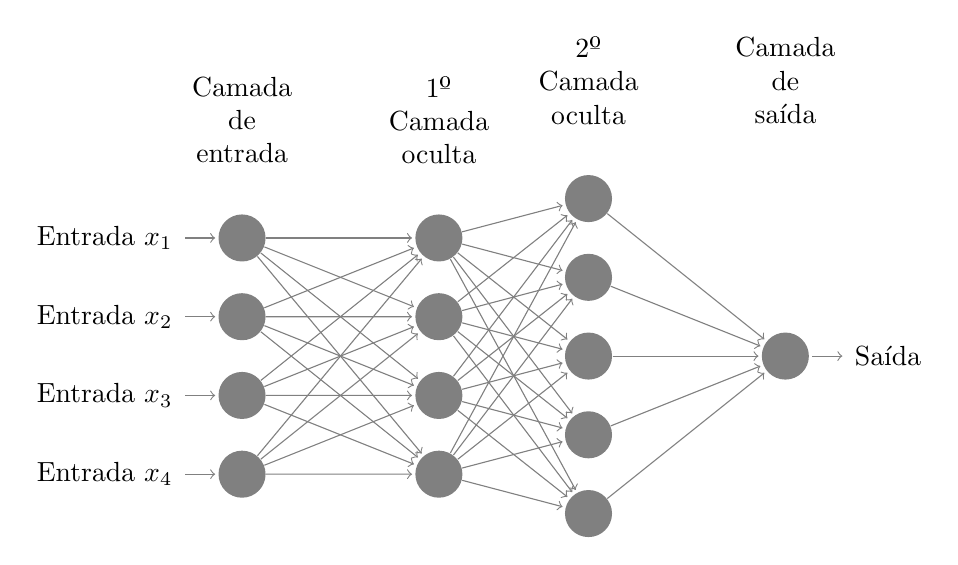
\begin{tikzpicture}[shorten >=1pt,->,draw=black!50, node distance=\layersep]
    \tikzstyle{every pin edge}=[<-,shorten <=1pt]
    \tikzstyle{neuron}=[circle,fill=black!25,minimum size=17pt,inner sep=0pt]
    \tikzstyle{input neuron}=[neuron, fill=black!50];
    \tikzstyle{output neuron}=[neuron, fill=black!50];
    \tikzstyle{hidden neuron}=[neuron, fill=black!50];
    \tikzstyle{annot} = [text width=4em, text centered]

    % Draw the input layer nodes
    \foreach \name / \y in {1,...,4}
    % This is the same as writing \foreach \name / \y in {1/1,2/2,3/3,4/4}
        \node[input neuron, pin=left:Entrada $x$$_\y$] (I-\name) at (0,-\y) {};

    % Draw the hidden layer nodes
    \foreach \name / \y in {1,...,4}
        \path[yshift=0cm]
            node[hidden neuron] (H-\name) at (\layersep,-\y cm) {};
            
    % Draw the second hidden layer nodes
    \foreach \name / \y in {1,...,5}
        \path[yshift=0.5cm, xshift=1.9cm ]
            node[hidden neuron] (J-\name) at (\layersep,-\y cm) {};

    % Draw the output layer node
    \node[output neuron,pin={[pin edge={->}]right:Saída}, right of=J-3] (O) {};

    % Connect every node in the input layer with every node in the
    % hidden layer.
    \foreach \source in {1,...,4}
        \foreach \dest in {1,...,4}
            \path (I-\source) edge (H-\dest);
   
   % Connect every node in the hidden layer 1 with every node in the
    % hidden layer 2.     
     \foreach \source in {1,...,4}
        \foreach \dest in {1,...,5}
            \path (H-\source) edge (J-\dest);

    % Connect every node in the hidden layer with the output layer
    \foreach \source in {1,...,5}
        \path (J-\source) edge (O);

    % Annotate the layers
    \node[annot,above of=H-1, node distance=1.5cm] (hl) {1º Camada \\ oculta};
    \node[annot,above of=J-1, node distance=1.5cm] (hl2) {2º Camada \\ oculta};
    \node[annot,left of=hl] {Camada de entrada};
    \node[annot,right of=hl2] {Camada de \\ saída};
    %\node[annot,above of=H-1, node distance=1.5cm] (hl) {Camada de \\ Saída};
\end{tikzpicture}
    \fonte{Adaptado de \citeonline{livroNunes2016}}
    \label{figure:multilayer_perc}
\end{figure}

\par Por fim, as redes recorrentes que recebem este nome por conta da realimentação entre os neurônios da mesma camada, ou seja, a saída de um neurônio em uma camada, pode servir como entrada para outro neurônio da mesma camada \cite{Nelson2017}.

\par Estas formas de organização presentes nas arquiteturas, estão intimamente relacionadas ao processo de aprendizado que é aplicado nas RNAs \cite{Haykin2001}.

\subsection{Processo de aprendizado}

\par Um dos pontos mais relevantes das RNAs é a generalização \cite{livroNunes2016}, onde treina-se levando em consideração um conjunto amostral \textit{A}, que faz uma boa representação do problema resolvido na tarefa e então após este processo a rede consegue realizar a tarefa não somente para o conjunto \textit{A}, mas também para um conjunto \textit{C} qualquer \cite{livroNunes2016}.

\par Porém para a generalização, como citado, é necessário um processo de treinamento, que seja adequado a arquitetura de RNA. \citeonline{livroNunes2016} definem processo de treinamento como um algoritmo que, através de passos bem definidos ajustam os pesos sinápticos da RNA com o objetivo de permitir o mapeamento das relações dos dados e então generalizar. 

\par Os processos de treinamento podem adotar diferentes estratégias para ensinar as RNAs, e cada estratégia gera um algoritmo de aprendizado diferente, sendo os principais, algorítimos de aprendizado supervisionado e não-supervisionado.

\par No aprendizado supervisionado, há rótulos $y^{(t)}$ que indicam o comportamento $\widehat{y}$ que a rede deve apresentar para cada $x^{(t)}$ presente em um conjunto de dados $\{(x^{(t)}, y^{(t)}): 1 \leqslant t \leqslant T\}$ \cite{bezerra2016}. Desta forma, de acordo com os resultados apresentados, ajustes são feitos nos pesos sinápticos e limiares dos neurônios da RNA \cite{livroNunes2016}, para que o resultado gerado seja o mais próximo possível de $y^{(t)}$ \cite{Osorio1999}. Assim, o objetivo do aprendizado supervisionado é gerar para uma entrada \textit{x}, um valor de \textit{y} próximo a $y^{(t)}$, sendo que, para valores categóricos de \textit{y}, tem-se uma classificação e para valores numéricos uma regressão \cite{murphy2012}.

\par Já o aprendizado não supervisionado, são utilizados apenas os dados, sem qualquer tipo de rótulo, sendo utilizados para gerar grupos \cite{Camila2017} e com isto descobrir novos padrões no conjunto de dados \cite{murphy2012}

\par Após a aplicação dos algoritmos de treinamento é necessário avaliar a performance do modelo de RNA gerado, para garantir que o mesmo está sendo capaz de generalizar. Uma maneira de realizar a avaliação é verificando a acurácia da RNA através da quantidade de acertos do modelo frente a um conjunto de dados não apresentado para a RNA durante o processo de treinamento, fazendo com que o conjunto de dados tenha de ser separado em dados de treino e teste \cite{Goodfellow-et-al-2016}.

\par A separação dos dados, pode ser utilizada também para a identificação de problemas de \textit{Underfitting}, que é causado quando o modelo não consegue extrair características relevantes do conjunto de dados, obtendo altas taxas de erro durante o treinamento, ou mesmo o \textit{Overfitting}, que ocorre quando o modelo extrair características além do necessário do conjunto de dados, fazendo assim com que o modelo tenha baixas taxas de erro no treino e praticamente não acerte no teste \cite{Goodfellow-et-al-2016}. Na Figura \ref{figure:over_under} os problemas expostos anteriormente são representados, onde (a) representa o \textit{Underfitting}, (c) \textit{Overfitting} e (b) o ideal. 

\image{0.87}{aprendizado/overfitting_under_editado.png}{Representação gráfica do \textit{Overfitting} e \textit{Underfitting}}{figure:over_under}{Adaptado de \citeonline{gibsonadampattersonjosh2017}}

\par Para muitos casos as RNAs são utilizadas pois conseguem chegar ao ideal (Figura \ref{figure:over_under} (b)) \cite{Goodfellow-et-al-2016}, garantindo assim a generalização, porém a depender do escopo do problema, as RNAs necessitam de mais camadas, cada uma delas com certas especialidades, para possibilitar a extração mais sofisticada de características do problema modelado pela RNA.

\section{Aprendizado Profundo}

\par O Aprendizado Profundo (AP) apresenta uma abordagem diferente para os problemas resolvidos com técnicas de RNA, onde múltiplas camadas são empregadas nas arquiteturas, permitindo assim que problemas mais complexos e sofisticados sejam mapeados \cite{Goodfellow-et-al-2016}.

\par As características dos algoritmos de AP fizeram com que estes chegassem ao estado-da-arte em diversos casos, como em \citeonline{Shankar2017} e \citeonline{Krizhevsky2012}. 

\subsection{Redes Neurais Convolucionais}

\par Redes Neurais Convolucionais (RNC) são uma variação das redes PMC, tendo sua criação inspirada no processo biológico de processamento de dados visuais \cite{Caroline2016}. Estas arquiteturas de AP, são capazes de subdividir os dados para tentar extrair características relevantes a classificação, reduzindo assim o números de parâmetros que deverão ser ajustados pela rede \cite{Miyazaki2017}, melhorando o processo de treinamento \cite{Miyazaki2017}.

\par As RNCs são utilizadas em problemas em que os dados tem estruturas de grade, como por exemplo, processamento de fala e entendimento da linguagem natural (Uma dimensão, convolução temporal) \cite{Miyazaki2017} e segmentação e classificação de imagens (Duas dimensões, convolução espacial) \cite{Miyazaki2017, Goodfellow-et-al-2016}.

\par Um dos primeiros modelos de RNCs propostos foi a LeNet \cite{LeCun1998} (Figura \ref{figure:lecun_basic}), formada por conjunto de camadas, também nomeada de blocos de funções, onde cada uma delas possui um objetivo específico \cite{Carneiro2017}.

\image{0.6}{cnn_lenet.JPG}{Estrutura básica de RNC proposta por \citeonline{LeCun1998} aplicado na identificação de tumores normais e anormais}{figure:lecun_basic}{\citeonline{Carneiro2017}}

\par As três camadas fundamentais para uma RNC, apresentadas por \citeonline{LeCun1998}, e ilustradas na Figura \ref{figure:lecun_basic}, são as seguintes: convolucional, de \textit{pooling} e totalmente conectada.

\subsubsection{Camada convolucional}

\par A camada convolucional representa um conjunto de filtros não lineares que percorrerem os dados de entrada sequencialmente e produzem os mapas de características \cite{Miyazaki2017}. O processo de percorrer os dados de entrada ocorre através de passos (\textit{strides}), passando de \textit{pixel} em \textit{pixel} nas imagens de entrada.

\par Nesta camada há dois conceitos centrais: o campo receptor local e o compartilhamento de pesos sinápticos. Assim, com o campo receptor local, ao contrário das RNAs tradicionais, na qual todo o volume de entrada é conectado a camada oculta, apenas uma região específica definida pelo compartilhamento de pesos sinápticos é retirada da camada de entrada \cite{mnielsen2018}.

\par A Figura \ref{figure:conv_complete} mostra o processo de convolução, onde, um filtro \textit{3}x\textit{3}, definido pelo compartilhamento dos pesos sinápticos, passa sobre uma região dos dados, com passo igual a \textit{1}, e a multiplicação entre eles é realizada, e os valores resultantes são somados e colocados no mapa de características.

\image{0.6}{conv_completa.png}{Processo de convolução}{figure:conv_complete}{Adaptado de \citeonline{pavlovskyvojtech2017}}

\par Com isto, no mapa de características há apenas características relevantes para a classificação.

\subsubsection{Rectified Linear Units}

\par Ao final da camada de convolução, normalmente aplica-se uma função de ativação \cite{Carneiro2017}, e a mais comumente utilizada para RNCs é a \textit{Rectified Linear Units} \cite{nair2010, Krizhevsky2012}. Essa função é calculada pela Equação \ref{form:relu}.

\begin{equation}
    f(x) = max(0, x)
\label{form:relu}
\end{equation}

\par Esta função faz com que, sejam passados para as camadas subsequentes a ela, apenas valores positivos, já que todos os negativos são substituídos por zero. 

\subsubsection{Camada de Pooling}

\par A camada de \textit{Pooling}, comumente utilizada após uma certa camada de convolução \cite{Caroline2016}, tem a finalidade de reduzir a dimensionalidade dos dados do mapa de características \cite{Caroline2016}. Esta redução é feita principalmente para agilizar o processo de treinamento \cite{Caroline2016}.

\par Esta redução é feita com o agrupamento de valores através de uma janela \textit{M}x\textit{N} que é passada pelo mapa de características, aplicando uma função, normalmente de média ou de valor máximo \cite{Amidi2018}. A Figura \ref{figure:pooling} apresenta uma operação de \textit{Pooling} feita através de um filtro 2x2, com a função de valor máximo.

\image{0.34}{pooling/pooling_v2.png}{Processo de \textit{Pooling}}{figure:pooling}{Adaptado de \citeonline{rawat2017}}

\par Segundo \citeonline{mnielsen2018}, o filtro de \textit{Pooling} normalmente é utilizado as dimensões 2x2 com um passo de deslocamento igual a 1.

\subsubsection{Camada totalmente conectada}

\par A saída das camadas convolucionais e de \textit{Pooling} geram as características extraídas dos dados de entrada \cite{Carneiro2017}. As camadas totalmente conectadas utilizam estas características para classificar os dados. As camadas totalmente conectadas representam uma PMC \cite{Haykin2001} descrita nos capítulos anteriores, mas, sua saída é controlada por uma função de ativação, normalmente \textit{softmax}, responsável pela classificação dos resultados \cite{Bishop2006}.

\subsubsection{Transferência de Aprendizado}

\par Realizar treinamentos de RNCs requer grandes quantidades de dados, não sendo comum realizar treinamento deste tipo de rede do zero \cite{Carneiro2017}, normalmente essas redes apresentam muitas camadas e realizar o ajuste de cada camada pode exigir muitos dados. Desta forma é comum utilizar modelos que já possuem parâmetros ajustados para outros conjuntos de dados \cite{Ponti2018}, ou seja, aplica-se um domínio geral em um domínio específico. Todo esse processo é nomeado de Transferência de Aprendizado.

\par De acordo com \citeonline{Ponti2018} existem diversas abordagens para a realização da transferência de aprendizado, sendo algumas delas: (i) Permitir que o algoritmo de treino ajuste todos os pesos presentes na rede com os novos dados, (ii) Congelar algumas camadas e assim limitar o número de parâmetros treinados pela rede, (iii) Adicionar mais camadas no modelo e realizar o treinamento somente destas novas camadas.

\par A escolha da abordagem de transferência pode variar de acordo com a similaridade do novo conjunto de dados em relação ao antigo e também a seu tamanho \cite{Carneiro2017}.

\subsection{MobileNet}

\par MobileNet é um modelo de RNC criado para apresentar bons resultados em classificações de imagens e ao mesmo tempo, ser leve, tanto no tamanho em memória, quanto no custo operacional de suas operações, isto para que seja possível realizar sua aplicação em \textit{Smartphones} e aplicações embarcadas de visão computacional. Faz isto através da aplicação de técnicas de convolução profunda separável, onde um filtro é aplicado para cada camada de cor, tornando o modelo mais leve \cite{howard2017mobilenets}.

\subsection{PoseNet}

\par PoseNet é um modelo de RNC, criado pelo \textit{Google Creative Lab} com base nos trabalhos \citeonline{george2017} e \citeonline{george2018} que realiza a identificação de 17 pontos do corpo humano (Figura \ref{figure:posenet_poses}), de um ou vários usuários.

\image{0.65}{figura_traduzida.jpg}{Pontos identificados pelo PoseNet}{figure:posenet_poses}{Adaptado de \citeonline{PoseNetMedium2019}}

\par Mesmo fazendo muitas identificações (Figura \ref{figure:posenet_poses}), o PoseNet é um modelo leve, o que permite sua aplicação em diversos contexto, como em aplicações \textit{web} e \textit{mobile} \cite{PoseNetMedium2019}.

\section{Conceitos Tecnológicos}

Nesta seção as tecnologias utilizadas durante a desenvolvimento do presente trabalho são expostas.

\subsection{Linguagens de Programação}

\par O processamento e coleta dos dados foi feito utilizando a linguagem de programação Python \cite{Python2019}, junto as bibliotecas OpenCV e scikit-image para o processamento das imagens, Augmentor, para a aplicação de modificações nas imagens no processo de \textit{Data Augmentation} e PyQt para a criação de interfaces gráficas.

\par A criação e treinamento dos modelos de RNCs aplicados nos RA utilizou Python junto a biblioteca Keras, que permite a criação em alto nível de RNAs profundas, além de disponibilizar modelos já treinados e funcionalidades para a aplicação de transferência de aprendizado \cite{chollet2015}. A disponibilização dos resultados do Keras é feita através de arquivos hierárquicos (H5), que podem ser consumidos por outras bibliotecas, como as presentes no ecossistema do TensorFlow.

\par Para o desenvolvimento da biblioteca de RAs, fez-se a utilização da linguagem de programação JavaScript, junto as bibliotecas, P5.js, para uma manipulação facilitada de DOM e TensorFlow.js (TFJS), para o desenvolvimento de Aprendizado Profundo na \textit{web}, isso além de permite a utilização de modelos de rede neural em navegadores, e também disponibiliza modelos já treinados \cite{tensorflowjs2019}, da mesma forma que o Keras.

\par Por fim, para a distribuição do modelo de rede neural treinado neste trabalho, fez-se uma \textit{API Rest} utilizando o \textit{Microframework web} de Python Flask, que permite a construção simplificada de aplicações \textit{web}.

\subsection{Google Colaboratory}

\par Colaboratory (Colab) é uma ferramenta criada pelo Google que permite a fácil execução de algoritmos de aprendizado de máquina. Colab é criado sob o pacote Jupyter, um ambiente interativo, executado no navegador, que permite a execução de linguagens interpretadas \cite{PER-GRA:2007}. Todo o ambiente do Colab é executado sobre máquinas aceleradas por \textit{Graphics Processing Unit} (GPU), o que diminui o tempo de execução de processos de treinamento de modelos de rede neural.
